\lab{1-D Optimization}{1-D Optimization}
\label{lab:1-dOpt}
\objective{
Many high-dimensional optimization algorithms rely on one-dimensional optimization methods.
In this lab, we implement four \emph{line search} algorithms for optimizing scalar-valued functions defined on $\mathbb{R}$.
We will generalize some of these approaches to high-dimensional optimization problems in subsequent labs.
% In some sense, they represent the simplest nontrivial case in general optimization, as there is only one parameter to optimize.
% Even so, many sophisticated optimization algorithms rely crucially on the effectiveness and efficiency of line searches, since higher-dimensional problems are often broken down into one-dimensional optimizations.
% There are many different one-dimensional optimization methods, and their effectiveness depends very much on the nature of the optimization problem.
% Although the line search procedure is often only a subroutine of the optimization algorithm at hand, understanding the basics of the line search is necessary for understanding the robustness of the entire algorithm.
% For some functions, we can use techniques from calculus to analytically obtain this minimizer.
% However, in practical applications, this is often impossible, especially when
% we need a system that works for a wide class of functions.
}

\section*{Overview of Line Search Algorithms} % ===============================

% TODO: make this metaphor WAY more concise.
Imagine you are hiking a steep mountain.
When it is time to head home, thick fog gathers around, reducing visibility to just a couple of feet.
How can you find your way back with such limited visibility?
One strategy is to pick a downhill direction and follow that direction as far as you can, or until it starts leading upward again.
Then choose another downhill direction, and take that as far as you can, repeating the process.
By always choosing a downhill direction, you hope to eventually make it back to the base of the mountain.

This is the basic approach of \emph{line search algorithms} for numerical optimization.
Let $f$ be a scalar-valued function.
The goal is to find the \emph{global minimizer} $\x^*$ such that $f(\x^*) \le f(\x)$ for all $\x$ in the domain of $f$.
After choosing an initial guess $\x_0$, we produce a sequence of approximations $\x_1,\ \x_2,\ \x_3,\ \ldots$ using the rule
\begin{equation}
    \x_{k+1} = \x_k + \alpha_k \mathbf{p}_k.
    \label{eq:line-search-iter}
\end{equation}
The point $\mathbf{p}_k$ is the \emph{search direction} (which way to go) and the scalar $\alpha_k$ is called the \emph{step size} (how far to go).
% This procedure is called a line search because at each iteration, we are simply examining the function in a particular linear direction.
% The choice of the step size $\alpha_k$ is often chosen by solving a one-dimensional optimization problem in the given direction.
The choice of search direction and step size at each step is what defines different line search algorithms.

\subsection*{Derivative versus Derivative-Free Methods} % ---------------------

A function's derivative provides information about how the value of the function changes at each point, and can be used to determine local optima.
Unfortunately, not all objective functions are differentiable, and many are difficult or costly to differentiate.
Thus some line search methods utilize the derivative of the objective function, but others do not.

\section*{Interval Approximation Methods for Unimodal Functions} % ============

A function $f:[a,b]\rightarrow\mathbb{R}$ satisfies the \emph{unimodal property} if it has just \textbf{one} local (hence global) minimum and is monotonic to the left and right of the minimum.
The following line search methods optimize a unimodal function by partitioning the function's domain into progressively smaller intervals that contain the minimizer.
% Although we may not end up with the exact minimum, these method allows us to pin down the true minimum within an interval of any given width in a finite number of steps.
% The first two, golden section and bisection search, are especially simple, as the step size in some sense is fixed, and we are only left with a binary decision of search direction.
% Newton's Method uses an algorithm to determine both the step size and direction of the search.
% Our final algorithm, The Secant Method, can be thought of as an approximation of Newton's Method.

\subsection*{Golden Section Search} % -----------------------------------------

Let $f:[a,b]\rightarrow\mathbb{R}$ be unimodal.
Starting with the closed interval $[a,b]$, the \emph{golden section search} finds a smaller interval that contains $x^*$ as follows.

Choose two points $a'$ and $b'$ with $a' < b'$.
If $f(a') \geq f(b')$, the unimodal property guarantees that the minimizer must be in the interval $[a', b]$, for otherwise the function $f$ would have a local minimum in both $[a, a']$ and $[a', b]$. % TODO: WHY??
In the next step, we repeat the process over the interval $[a', b]$.
If instead $f(a') \leq f(b')$, then we choose the interval $[a, b']$ for the next step.
Finally, if $f(a') = f(b')$, then it does not matter which interval is chosen.

It turns out that there is an optimal choice for the two test points $a'$ and $b'$.
Given the current interval $[a, b]$, choose $a'$ and $b'$ satisfying
\begin{align*}
a' &= a + \rho(b - a) \\
b' &= a + (1 - \rho)(b - a),
\end{align*}
where $\rho = \frac{1}{2}(3 - \sqrt{5}) \approx 0.382$ (this constant is related to the famous \emph{golden ratio}, hence the name of the algorithm).

\begin{comment} % TODO: What does this have to do with the implementation?
By choosing these particular points, we need to only evaluate the function at one additional point in the next step.
To demonstrate this fact, the reader may verify that, within the interval $[a, b']$, the point $a'$ already satisfies the equation
\begin{equation*}
a' = a + (1 - \rho)(b' - a),
\end{equation*}
and so we need only evaluate the function at the point $c$ satisfying
\begin{equation*}
c = a + \rho(b' - a).
\end{equation*}
\end{comment}

At each step, the interval is reduced by a factor of $1-\rho$, which means that after $n$ steps, the minimizer is pinned down to within an interval approximately $(0.618)^n$ times the length of the original interval.
Note that this rate of convergence is independent of the objective function.

\begin{problem} % Golden Section Search
Write a function that accepts a callable function $f$, interval limits $a$ and $b$, and a number of iterations \li{niter} to calculate.
Implement the golden section search as described above, returning the midpoint of the final interval.

Use your function to minimize $f(x) = e^x - 4x$ on the interval $\lbrack 0, 3 \rbrack$.
How many steps do you need to take to get within $.001$ of the true minimizer?
% TODO: how do you plan on testing / reporting this part?
\label{prob:golden-section-search}
\end{problem}

\subsection*{Bisection Algorithm} % -------------------------------------------

This method is similar to the Golden Ratio method, but instead of cutting our interval into two overlapping sections, we divide the interval evenly in half, and then use the derivative $f'(x)$ to determine where the minimizer lies.
This method takes advantage of the fact that a unimodal function's derivative is strictly less than 0 to the left of the minimizer, and strictly greater than 0 to the right.

For a unimodal function $f:[a, b]\rightarrow\mathbb{R}$, take the midpoint, $x_1 = \frac{b + a}{2}$.
If $f'(x_1) > 0$, the critical point must lie in the interval $[a, x_1]$; otherwise, the critical point lies in the other half of the interval, $[x_1, b]$.
We repeat this process on the correct interval until the desired accuracy is achieved.

At each step, the interval is reduced by a factor of two.
This is slightly quicker than the factor of $1-\rho$ in the Golden Section search method.
Like the golden section search, the convergence of this method is independent of the objective function.

\begin{problem} % Bisection algorithm
Write a function that accepts a callable function $f$, interval limits $a$ and $b$, and a number of iterations \li{niter} to calculate.
Implement the bisection algorithm as described above, returning the midpoint of the final interval.

Use your function to minimize the same objective function as in Problem \ref{prob:golden-section-search}.
How many steps do you need to take to get within $.001$ of the true minimizer?
Time both algorithms and report which one is faster to converge.
% TODO: how do you plan on testing this?
\end{problem}

\section*{Newton's Method and Quasi-Newton Methods} % =========================

Newton's Method, is a basic line search algorithm that uses the derivatives of the function to select a direction and step size.

To use this method, we need a function that is twice differentiable.
The idea is to approximate the function with a quadratic polynomial and then solve the trivial problem of minimizing the polynomial.
Doing so in an iterative manner can lead us to the actual minimizer.
Let $f$ be a function satisfying the appropriate conditions, and let us make an initial guess, $x_0$.
The relevant quadratic approximation to $f$ at $x_0$ is
\begin{equation*}
q(x) = f(x_0) + f'(x_0)(x-x_0) + \frac{1}{2}f''(x_0)(x-x_0)^2,
\end{equation*}
which is the second-degree Taylor polynomial for $f$ centered at $x_0$.
The minimum for this quadratic function is easily found by solving $q'(x) = 0$, and we take the obtained $x$-value as our new approximation.
The formula for the $(k+1)$-th approximation, which the reader can verify, is
\begin{equation*}
x_{k+1} = x_k - \frac{f'(x_k)}{f''(x_k)}.
\end{equation*}
In the one dimensional case, there are only two search directions: to the right ($+$) or to the left ($-$).
Newton's method chooses the search direction $\p_k = \text{sign}(-f'(x_k)/f''(x_k))$ and the step size $\alpha_k = |f'(x_k)/f''(x_k)|$.

The convergence properties of this sequence depend heavily on the initial guess $x_0$ and the function $f$.
Roughly speaking, if $x_0$ is sufficiently close to the actual minimizer, and if $f$ is well-approximated by parabolas, then one can expect the sequence to converge quickly.
However, there are cases when the sequence converges slowly or not at all.
See Figure \ref{linesearch:newton}.

\begin{figure}
\centering
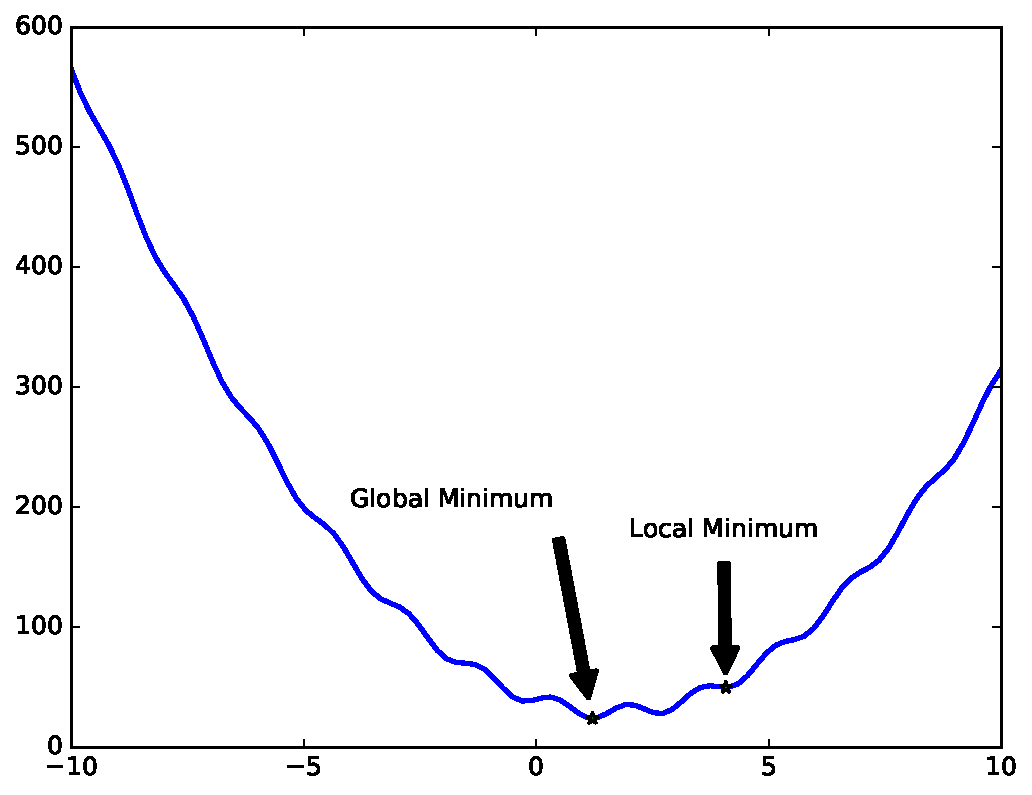
\includegraphics[width=.7\textwidth]{newton.pdf}
\caption{The results of Newton's Method using two different initial guesses.
The global minimizer was correctly found with initial guess of 1.
However, an initial guess of 4 led to only a local minimum.}
\label{linesearch:newton}
\end{figure}

\begin{problem}
Implement Newton's Method.
You will write a function that takes a function and its two derivatives, as well as a starting point.
It will return the minimizer.

Use this function to minimize $f(x) = x^2 + \sin(5x)$ with an initial guess of $x_0 = 0$.
Now try other initial guesses farther away from the true minimizer, and note when the method fails to obtain the correct answer.
\end{problem}

\subsection*{One-Dimensional Secant Method} % ---------------------------------

Sometimes we would like to use Newton's Method, but for whatever reason we don't have a second derivative.
Maybe calculating it is too costly or the function is not twice differentiable.
In this situation we can approximate the second derivative using the first derivative.
The approximation using a secant calculation, hence the name.
We use the same basic algorithm as in Newton's Method, but with an approximation for the second derivative of the objective function.
\begin{equation*}
x_{n+1} = x_n - \frac{f'(x_n)}{f''_{approx}(x_n)},
\end{equation*}
where we approximate the second derivative as follows:
\begin{equation*}
f''_{approx}(x_n) = \frac{f'(x_n) - f'(x_{n-1})}{x_n - x_{n-1}}.
\end{equation*}
This gives us the final equation:
\begin{equation*}
x_{n+1} = x_n - \frac{x_n - x_{n-1}}{f'(x_n) - f'(x_{n-1})}f'(x_n),
\end{equation*}
Notice that this equation requires two initial points (both $x_n$ and $x_{n-1}$) to calculate the next estimate.

\begin{problem}
Implement the Secant Method.
You will write a function that accepts a function, its first derivative and a starting point, and returns the function's minimizer.

Use this function to minimize $x^2 + \sin(x) + \sin(10x)$ with an initial guess of $x_0 = 0$.
Now try other initial guesses farther away from the true minimizer, and note when the method fails to obtain the correct answer.

(Hint: You may want to plot this function to understand why this problem is so sensitive to the starting point.)
\end{problem}

\section*{General Line Search Methods} % ======================================

\subsection*{Step Size Calculation} % -----------------------------------------

Given a differentiable function $f: \mathbb{R}^n \rightarrow \mathbb{R}$ that we wish to minimize, and assuming that we already have a current point $\x_k$ and direction $\p_k$ in which to search, how do we choose our step size $\alpha_k$? If our step size is too small, we will not make good progress toward the minimizer, and convergence will be slow.
If the step size is too large, however, we may overshoot and produce points that are far away from the solution.
A common approach to pick an appropriate step size involves the \emph{Wolfe conditions}:

\begin{align*}
&f(\x_k + \alpha_k\p_k) \leq f(\x_k) + c_1\alpha_k\nabla f(\x_k)\trp \p_k, &(0 < c_1 < 1),
\\ &\nabla f(\x_k + \alpha_k\p_k)\trp \p_k \geq c_2\nabla f(\x_k)\trp \p_k, &(c_1 < c_2 < 1).
\end{align*}

The search direction $p_k$ is often required to satisfy $p_k\trp \nabla f(\x_k) < 0$, in which case it is called a \emph{descent direction}, since the function is guaranteed to decrease in this direction.
Generally speaking, choosing a step size $\alpha_k$ satisfying these conditions ensures that we achieve sufficient decrease in the function and also that we do not terminate the search at a point of steep decrease (since then we could achieve even better results by choosing a slightly larger step size).
The first condition is known as the \emph{Armijo} condition.

We will discuss methods of finding search directions in future labs.
For now, we will discuss one simple algorithm for finding an appropriate step size which satisfies the Armijo conditions.

\subsection*{Backtracking} % --------------------------------------------------

Finding such a step size satisfying these conditions is not always an easy task, however.
One simple approach, known as \emph{backtracking}, starts with an initial step size $\alpha$, and repeatedly scales it down until the Armijo condition is satisfied.
That is, choose $\alpha >0, \rho \in (0, 1), c\in (0, 1)$, and while
\[f(\x_k + \alpha \p_k) > f(\x_k) + c\alpha\nabla f(\x_k)\trp \p_k,\]
re-scale $\alpha = \rho\alpha$.
Once the loop terminates, set $\alpha_k = \alpha$.
Note that the value $\nabla f(\x_k)\trp \p_k$ remains fixed for the duration of the backtracking algorithm, and hence need only be calculated once at the beginning.

\begin{problem} % Backtracking
Implement this backtracking algorithm using the function definition in the spec file.
Your function will accept a function, its derivative, a starting point, and the direction p.
\end{problem}

% TODO: Need a problem that USES this backtracking algorithm!

\subsection*{Line Search in SciPy} % ------------------------------------------

SciPy's \li{optimize} module contains implementations of various optimization algorithms, including several line search methods.
In particular, the module provides a useful routine for calculating a step size satisfying the Wolfe Conditions described above, which is more robust and efficient than our simple backtracking approach.
We recommend its use for the remainder of this lab.
The function is called \li{line_search()}, and accepts several arguments.
We can typically leave the keyword arguments at their default values, but we do need to pass in the objective function, its gradient, the current point, and the search direction.
The following code gives an example of its usage, using the objective function $f(x, y) = x^2+4y^2$.

\begin{lstlisting}
>>> import numpy as np
>>> from scipy.optimize import line_search
>>>
>>> def objective(x):
>>>     return x[0]**2 + 4*x[1]**2
>>>
>>> def grad(x):
>>>     return np.array([2*x[0], 8*x[1]])
>>>
>>> x = np.array([1., 3.]) # current point
>>> p = -grad(x)           # current search direction
>>> a = line_search(objective, grad, x, p)[0]
>>> print a
0.125649913345
\end{lstlisting}

Note that the function returns a tuple of values, the first of which is the step size.

% TODO: Needs an application problem that uses SciPy!
